\begin{figure}[H]
\centering
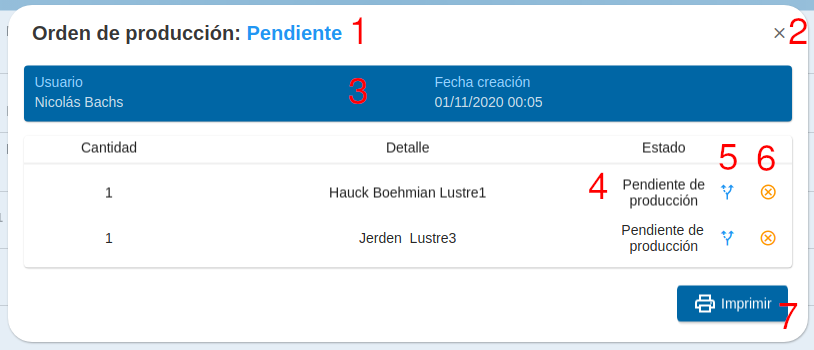
\includegraphics[width=\textwidth,height=\textheight,keepaspectratio]{Escenarios/AD-25-00}
\caption{Escenario - AD-25-00}
\label{fig:AD-25-00}
\end{figure}

Este escenario permite a un usuario visualizar una orden de producción, en \textbf{AD-25-01} se puede ver el estado de la orden de producción. Con el botón \textbf{AD-25-02} se puede cerrar la ventana, volviendo al escenario \textbf{AD-22-00}. En \textbf{AD-25-03} se muestra información acerca del empleado que creó la orden de producción y la fecha de creación. En \textbf{AD-25-04} se muestra el detalle de la orden de producción, donde se puede observar la cantidad a producir de un determinado mueble. También se muestra el estado en el cual se encuentra cada una de estas líneas. El botón \textbf{AD-25-05} permite ver las tareas asociadas a la orden de producción, navegando al escenario \textbf{AD-27-00} y el botón \textbf{AD-25-06} permite cancelar la linea de orden de producción indicada. Con el botón \textbf{AD-25-07} se podrá visualizar el PDF de la orden de producción, navegando al escenario \textbf{AD-26-00} teniendo la opción de imprimir.
\clearpage
